\documentclass[]{beamer}
\usetheme{Berlin}
\usepackage{tikz}
\usepackage{pgf-pie}
\usepackage{booktabs}
\usetikzlibrary {shadows}
% \usepackage{xcolor}

% \setlength{\arrayrulewidth}{0.5mm}

\title[]{Lab 4 Presentation}
\author{SeventeenEightyseven}
\institute{IIT Bombay}

% \setbeamercolor{block body example}{bg=green!100!yellow!30}

\begin{document}
\begin{frame}

\titlepage

\end{frame}

\begin{frame}
\frametitle{Topics to cover}
\tableofcontents
\end{frame}

\section{Important Theorem}
\begin{frame}
\frametitle{Important Theorem}
\begin{block}{Newton Second law \footnotemark}
\footnotetext[1]{This is the standard way of reference}
\emph{
Acceleration of a body is directly proportional to the force applied
on it and inversely proportional to the mass of the body. This
theorem derives the equation}
$$F=ma$$
\end{block}
\pause
% \begin{example}[Pythagorean theorem]
% $$h^2=p^2+b^2$$
% \end{example}
\begin{exampleblock}{Theorem (Pythagorean theorem)}
$$h^2=b^2+p^2$$
\end{exampleblock}
\end{frame}


\section{Match Result}
\begin{frame}
\frametitle{Cricket Result}
\begin{columns}
\column{0.3\textwidth}
\textbf{Team 1}
\begin{enumerate}
\item India
\item Pakistan
\item Bangladesh
\end{enumerate}
\column{0.3\textwidth}
\textbf{Team 2}
\begin{enumerate}
\item Australia
\item South Africa
\item West Indies
\end{enumerate}
\column{0.3\textwidth}
\textbf{Result}
\begin{enumerate}
\item India Won
\item South Africa won
\item Bangladesh won
\end{enumerate}
\end{columns}
\end{frame}


\section{My Expenses}
\begin{frame}{Semester expenses}
% My expenses
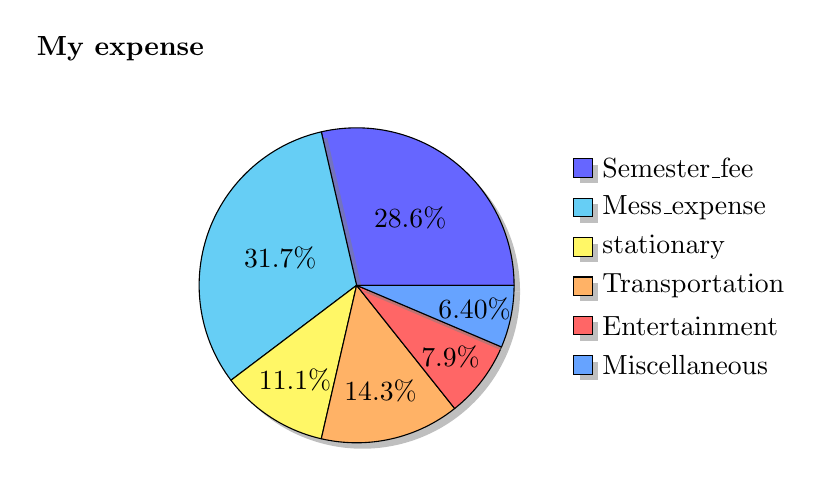
\begin{tikzpicture}

\pie[ pos={3,-3} , radius =2 , text=legend , style=drop shadow]{28.6/Semester\_fee , 31.7/Mess\_expense , 11.1/stationary , 14.3/Transportation , 7.9/Entertainment , 6.40/Miscellaneous }

\node[] {\textbf{My expense}};

\end{tikzpicture}
\end{frame}


\section{Important Formula}
\begin{frame}{XOR gate}

\begin{table}[]
    \centering
        \begin{tabular}{ c c c }
         \toprule
         \textbf{X} & \textbf{Y} & \textbf{Z} \\
         \hline
         FALSE & FALSE & FALSE \\ 
         FALSE & TRUE & TRUE \\ 
         TRUE & FALSE & TRUE \\
         TRUE & TRUE & FALSE \\
         \bottomrule
\end{tabular}
    \caption{Truth Table}
    \label{tab:label}
\end{table}
\end{frame}
\begin{frame}

\begin{center}
\Huge{The End}
\end{center}

\end{frame}

\end{document}
